\documentclass[12pt, twoside]{article}
\usepackage[letterpaper, margin=1in, headsep=0.5in]{geometry}
\usepackage[english]{babel}
\usepackage[utf8]{inputenc}
\usepackage{amsmath}
\usepackage{amsfonts}
\usepackage{amssymb}
\usepackage{tikz}
\usetikzlibrary{quotes, angles}
\usepackage{graphicx}
%\usepackage{pgfplots}
%\pgfplotsset{width=10cm,compat=1.9}
%\usepgfplotslibrary{statistics}
%\usepackage{pgfplotstable}
%\usepackage{tkz-fct}
%\usepackage{venndiagram}
\usepackage{enumitem}
\usepackage{multicol}


\usepackage{fancyhdr}
\pagestyle{fancy}
\fancyhf{}
\fancyhead[LE]{\thepage}
\fancyhead[RO]{\thepage \\Name: \hspace{4cm} \,\\}
\fancyhead[LO]{BECA / Dr. Huson / Geometry 10th Grade\\* Unit 10: Trigonometry \& analytic geometry \\ 12 March 2020}

\renewcommand{\headrulewidth}{0pt}

\begin{document}
\subsubsection*{10.4 Do Now: Linear equations, review}
  \begin{enumerate}

  \item Write down the slope perpendicular to the given slope. \vspace{0.5cm}
  \begin{enumerate}
    \begin{multicols}{2}
    \item   $m= -\frac{4}{3} \hspace{1cm} m_{\perp} = $
    \item   $m= 1.25 \hspace{1cm} m_{\perp} = $ 
    \end{multicols}
  \end{enumerate} \vspace{1cm}

  \item Write down the center and radius of each circle. Simplify radicals.
  \begin{enumerate}
    \begin{multicols}{2}
    \item   $(x+3)^2+(y-2)^2=25$ \vspace{2cm}
    \item   $(x-1)^2+y^2=48$
    \item   $x^2-4x+y^2-12y=9$ \vspace{2cm}
    \item   $x^2+y^2-18y=-17$
    \end{multicols}
  \end{enumerate}  \vspace{2cm}

  In the following problems, use the point-slope formula: $y-y_1=m (x-x_1)$
  \item What is the equation of a line through $(1,7)$ parallel to the line $y=\frac{3}{5}x-3$?  \vspace{2cm}
  \item What is the equation of a line through $(1,0)$ perpendicular to the line $4x-2y=8$?  \vspace{3cm}
  
  \item What is an equation of the perpendicular bisector of $\overline{AB}$ with $A(2,7)$ and $B(-4,-5)$? \vspace{2cm}

\newpage

\item $\triangle ABC$ is shown with $m\angle C=90^\circ$ and the lengths of the triangle's sides are $BC=5$, $AC=12$, and $AB=13$. (not drawn to scale)
  \begin{multicols}{2}
        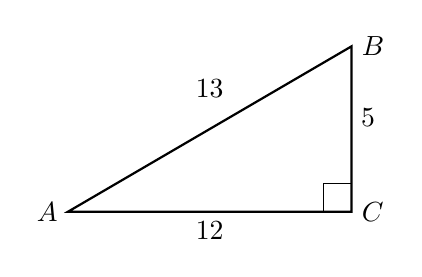
\begin{tikzpicture}[scale=0.6]
          \draw [thick]
          (0,0)node[left]{$A$}--
          (6,0)node[ right]{$C$}--
          (6,3.5)node[right]{$B$}--cycle;
          \draw (6,0)++(-0.6,0)--++(0,0.6)--+(0.6,0);
          \node at (3,0)[below]{$12$};
          \node at (6,2)[right]{$5$};
          \node at (3,2.2)[above]{$13$};
        \end{tikzpicture}
        \begin{enumerate}
        \item Write down the value of $\tan A$.  \\ \hfill [1 mark]\vspace{0.5cm}
        \item Find the measure of $\angle A$.  \hfill [2 marks] \vspace{1cm}
      \end{enumerate}
    \end{multicols} \vspace{2cm}

\item The following diagram shows a pole BT 1.6 m tall on the roof of a vertical building. \\[0.25cm]
  The angle of elevation of the top of the building from A is  
  $30^\circ$ and the distance from point $A$ to the building is 50 feet. 
    \begin{center}
      \begin{tikzpicture}[scale=0.4]
        %\draw [-, thick] (0,0)--(35:23);
        \draw [-, thick] (-4,0)--
        (0,0)--
          (17,0)--
          (22,0)--
          (22,10)--(17,10) node[left]{$B$};
        \draw [-, thick] (17,0)--(17,12)node[left]{$T$};
        \draw [fill] (0,0) circle [radius=0.1] node[below]{$A$};
        \draw [dashed] (0,0)--(17,10);
        \node at (3, 0)[above]{$30^\circ$};
        \node at (-3, 0)[below]{ground};
        \node at (19.5, 5)[above]{building};
      \end{tikzpicture}
      \end{center}
      Find the height of the building to the \emph{nearest foot}.

\end{enumerate}
\end{document}

